\chapter{Entwurfsmuster}

%% https://en.wikipedia.org/wiki/Software_design_pattern
%% TODO vlt lieber Decorator Pattern https://de.wikipedia.org/wiki/Decorator vlt die Wrapper?
\section{Singleton}

Das Singleton wurde für die beiden Klassen MariaDBConnector und JWTProvider eingesetzt.
Hierbei wurde eine Lazy Instantiation eingesetzt da dadurch die Systemstartzeit nicht verlängert wird.
Es wurde keine Synchronized Lazy Instantiation eingesetzt, da sowieso alles auf dem selben Thread läuft.

\subsection{Einsatz begründen}

Das Singleton kam zum Einsatz da es gerantiert,
dass Systemweit nur eine Instanz vorhanden ist und es zum nur eine einheitliche aktive Datenbank Verbindung und eine JWTProvider Instanz geben soll.
Zudem benötigt das System auch nur eine globale Instanz des JWTProvider.
Weiterhin ermöglicht es einen einfachen Zugriff auf diese Instanz, ist einfach zu verstehen und anzuwenden.
Und eine Instanz wird auch nur angelegt wenn diese auch benötigt wird.
Durch das Singleton gibt es zwar keine Möglichkeiten für polymorpe Aufrufe mehr aber diese werden in diesem Fall auch nicht benötigt.

\newpage
\subsection{UML}


\begin{figure}[htbp]
    \centering
    \fbox{
        
\includegraphics[width=4cm]{MariaDBConnector_before}
        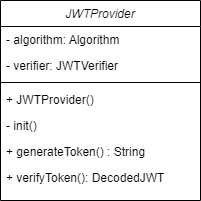
\includegraphics[width=4cm]{JWTProvider_before}
    }
    \caption{\label{1} UML vor Singleton}
\end{figure}

\begin{figure}[htbp]
    \centering
    \fbox{
        
\includegraphics[width=4cm]{MariaDBConnector_after}
        
\includegraphics[width=4cm]{JWTProvider_after}
    }
    \caption{\label{2} UML nach Singleton}
\end{figure}

